\documentclass[11pt,a4paper]{article}

% ---------- packages ----------
\usepackage[margin=2.2cm]{geometry}
\usepackage[utf8]{inputenc}
\usepackage{amsmath,amssymb}
\usepackage{graphicx}
\usepackage{booktabs}
\usepackage{tabularx}
\usepackage{array}
\usepackage{float}
\usepackage{caption}
\usepackage{enumitem}
\usepackage{xcolor}
\usepackage{listings}
\usepackage{titlesec}
\usepackage{fancyhdr}
\usepackage{enumitem}
\usepackage[colorlinks=true,linkcolor=blue!50!black,urlcolor=blue!50!black]{hyperref}

\graphicspath{{figures/}}
\captionsetup{font=small,labelfont=bf}
\setlist{itemsep=2pt,topsep=4pt}
\setlength{\parindent}{0pt}
\setlength{\parskip}{6pt}
\renewcommand{\arraystretch}{1.15}

\titleformat{\section}{\large\bfseries\color{black!40!black}}{\thesection}{0.6em}{}
\titleformat{\subsection}{\normalsize\bfseries\color{blue!40!black}}{\thesubsection}{0.6em}{}

\pagestyle{fancy}
\fancyhf{}
\renewcommand{\headrulewidth}{0pt}
\cfoot{\footnotesize Assignment 2 -- CNN from scratch on MNIST -- page \thepage}

\lstset{
  basicstyle=\ttfamily\footnotesize,
  backgroundcolor=\color{black!4},
  frame=single, rulecolor=\color{black!15},
  breaklines=true, columns=fullflexible, keepspaces=true,
  xleftmargin=2pt, xrightmargin=2pt
}

\newcommand{\code}[1]{\texttt{#1}}

% ---------- title ----------
\title{\textbf{CNN From Scratch on MNIST}}
\author{Kanika Montha \\ Student ID: a1985659}
\date{}

\begin{document}
\maketitle
\thispagestyle{fancy}

% =====================================================
\section{Implementation Summary}
This report explains, step by step, how I implemented a convolutional neural network (CNN) for MNIST digit classification using only NumPy. The forward pass, backward pass (backpropagation), loss function and mini-batch SGD optimiser are written by hand; no PyTorch or TensorFlow CNN layers are used (\code{torchvision} is used only to download the dataset). The convolution is evaluated efficiently with an \textbf{im2col / col2im} transformation. The final model reaches \textbf{97.44\% test accuracy} after 5 epochs, above the 94--96\% target in the brief.

\begin{table}[H]
\centering
\begin{tabularx}{\linewidth}{@{}l X@{}}
\toprule
\textbf{Item} & \textbf{Value} \\
\midrule
Architecture & Input $1{\times}28{\times}28$ $\to$ Conv(6, $3{\times}3$) $\to$ ReLU $\to$ MaxPool $2{\times}2$ $\to$ Conv(16, $3{\times}3$) $\to$ ReLU $\to$ MaxPool $2{\times}2$ $\to$ Flatten(400) $\to$ FC(128) $\to$ ReLU $\to$ FC(10) $\to$ Softmax \\
Training & Mini-batch SGD, batch size 32, learning rate 0.01, 5 epochs, softmax cross-entropy loss \\
Data split & 48{,}000 train / 12{,}000 validation (80/20 of the 60k training images) / 10{,}000 test \\
Trainable parameters & 53{,}558 \\
Selected model & Epoch 5 (highest validation accuracy, 96.84\%) \\
Test accuracy / loss & 97.44\% / 0.0856 (256 errors out of 10{,}000) \\
\bottomrule
\end{tabularx}
\end{table}

% =====================================================
\section{Data loading and preprocessing}
MNIST contains 70{,}000 greyscale images of handwritten digits ($28{\times}28$ pixels).
\begin{itemize}
  \item \textbf{Load} the 60{,}000 training and 10{,}000 test images with \code{torchvision.datasets.MNIST} and convert them to NumPy arrays.
  \item \textbf{Normalise} pixel values from $[0,255]$ to $[0,1]$ (divide by 255, float32). Small, consistently scaled inputs keep activations and gradients well-behaved for SGD with a fixed learning rate.
  \item \textbf{Reshape} to $(N,1,28,28)$, i.e.\ (batch, channels, height, width).
  \item \textbf{Split}: the 60{,}000 training images were shuffled with a fixed seed (42) and split 80/20 into 48{,}000 training and 12{,}000 validation images. The 10{,}000-image test set is kept untouched until the final evaluation.
\end{itemize}

\begin{figure}[H]
\centering
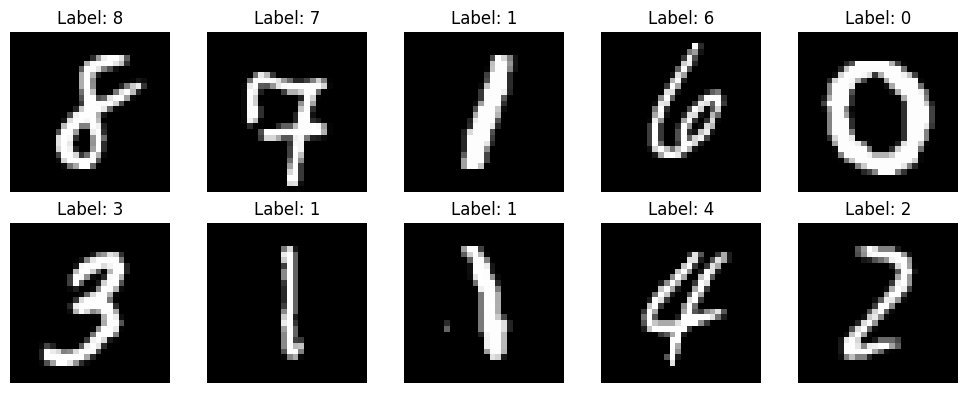
\includegraphics[width=0.8\linewidth]{fig_samples.png}
\caption{Sample training images with their labels.}
\end{figure}

% =====================================================
\section{Network architecture and tensor shapes}
The convolutions are ``valid'' (stride 1, no padding), so each $3{\times}3$ convolution reduces height and width by 2; each $2{\times}2$ pooling halves them, rounding down. A shape test with a dummy batch confirmed the expected sizes at every stage before training.

\begin{table}[H]
\centering
\begin{tabular}{@{}llr@{}}
\toprule
\textbf{Layer} & \textbf{Output shape} & \textbf{Parameters} \\
\midrule
Input & $1{\times}28{\times}28$ & 0 \\
Conv $3{\times}3$, 6 filters (+ReLU) & $6{\times}26{\times}26$ & $6\cdot(1\cdot3\cdot3)+6=60$ \\
MaxPool $2{\times}2$, stride 2 & $6{\times}13{\times}13$ & 0 \\
Conv $3{\times}3$, 16 filters (+ReLU) & $16{\times}11{\times}11$ & $16\cdot(6\cdot3\cdot3)+16=880$ \\
MaxPool $2{\times}2$, stride 2 & $16{\times}5{\times}5$ & 0 \\
Flatten & 400 & 0 \\
Fully connected 128 (+ReLU) & 128 & $400\cdot128+128=51{,}328$ \\
Fully connected 10 (softmax) & 10 & $128\cdot10+10=1{,}290$ \\
\midrule
\textbf{Total} & & \textbf{53,558} \\
\bottomrule
\end{tabular}
\end{table}

\textbf{Odd size handling.} The second convolution outputs $11{\times}11$ maps. A $2{\times}2$ stride-2 window fits 5 times, so the pooled output is $5{\times}5$ and the last row and column are ignored, giving $16\cdot5\cdot5=400$ features.

% =====================================================
\section{The im2col / col2im transformation}
This is part of calculation technique in convolutional layer. The purpose is to make convolution fast by turning it into matrix multiplication. A convolution slides a small kernel over the image and takes a dot product at every position. Doing this with Python loops would be far too slow, so the convolution layer uses \textbf{im2col} to turn it into a single matrix multiplication.

\begin{itemize}
  \item \textbf{im2col (forward pass):} copy every $3{\times}3$ patch of the input into one row of a matrix \code{cols}, and flatten each filter into one row of a matrix \code{W\_col}. Then \code{cols @ W\_col.T} computes the outputs for all images, positions and filters at once.
  \item \textbf{col2im (backward pass):} the reverse step. The gradient arrives as one row per patch and must be put back into image shape. Patches overlap, so each pixel's gradient is the \emph{sum} of the gradients from every patch that contains it; col2im places the patch gradients back and adds up the overlaps.
\end{itemize}

The cost is memory: because overlapping pixels are copied into several rows, the patch matrix is about 9 times larger than the image for $3{\times}3$ kernels.
% =====================================================
\section{Implementing the layers (forward and backward)}
Every layer is a small class with a \code{forward} method, which caches what the backward pass needs, and a \code{backward} method, which receives the gradient of the loss with respect to the layer's output and returns the gradient with respect to its input (storing weight gradients on the way). Backpropagation is simply calling \code{backward} through the layers in reverse order (the chain rule).

\subsection{Convolution layer}
\textbf{Forward:} im2col gives \code{cols}; the output is \code{cols @ W\_col.T + b}, reshaped to $(N,F,\text{out\_h},\text{out\_w})$.

\textbf{Backward:} the incoming gradient is reshaped to one row per patch (\code{dout\_rows}, shape $(N\cdot\text{out\_h}\cdot\text{out\_w},\,F)$). Then:
\begin{itemize}
  \item $\mathbf{db}$ = sum of \code{dout\_rows} over all rows (the bias was added at every position);
  \item $\mathbf{dW}$ = \code{dout\_rows.T @ cols}, reshaped to $(F,C,k,k)$: each weight's gradient accumulates (patch pixel $\times$ output gradient) over all positions and images;
  \item $\mathbf{dx}$: first \code{dcols = dout\_rows @ W\_col} (the gradient for every patch), then \textbf{col2im} folds it back to the input shape, summing overlaps.
\end{itemize}
\begin{lstlisting}[language=Python]
db = dout_rows.sum(axis=0)
dW = (dout_rows.T @ cols).reshape(W.shape)
dx = col2im(dout_rows @ W_col, x_shape, k, k, stride, padding)
\end{lstlisting}

\subsection{ReLU}
Forward: $\text{out}=\max(0,x)$, caching the mask $(x>0)$. Backward: $dx = dout \odot \text{mask}$, since the derivative of ReLU is 1 for positive inputs and 0 otherwise.

\subsection{Max pooling ($2{\times}2$, stride 2)}
\textbf{Forward:} the $(N,C,H,W)$ input is reshaped to $(N\cdot C,1,H,W)$ so each channel is processed separately, then im2col extracts the $2{\times}2$ windows as rows of length 4. \code{argmax} over each row finds the index of the maximum, and the row maximum is the output.

\textbf{Backward:} only the position that held the maximum influenced the output, so a zero matrix \code{dcols} is created and each upstream gradient is written at the stored argmax position; col2im then restores the image layout. All non-maximum positions receive zero gradient.
\begin{lstlisting}[language=Python]
cols, out_h, out_w = im2col(x.reshape(N*C, 1, H, W), p, p, stride, 0)
argmax = np.argmax(cols, axis=1);  out = cols[np.arange(len(cols)), argmax]
# backward:  dcols[np.arange(len(dcols)), argmax] = dout.reshape(-1);  dx = col2im(dcols, ...)
\end{lstlisting}

\subsection{Flatten and fully connected layers}
Flatten reshapes $(N,16,5,5)$ to $(N,400)$; its backward pass reshapes the gradient back. A fully connected layer computes $\text{out}=xW+b$ with gradients
\[
\mathbf{dW}=x^{\top}dout,\qquad \mathbf{db}=\sum_{n}dout_n,\qquad \mathbf{dx}=dout\,W^{\top}.
\]

\subsection{Weight initialisation}
Convolution weights and the first fully connected layer use \textbf{He initialisation} (normal with standard deviation $\sqrt{2/\text{fan\_in}}$), which keeps the variance of activations roughly constant through ReLU layers. The output layer has no ReLU after it, so it uses the smaller scale $\sqrt{1/\text{fan\_in}}$. Biases start at zero.

% =====================================================
\section{Softmax, cross-entropy and SGD}
\textbf{Softmax.} The last layer outputs 10 logits $z$; softmax gives probabilities
\[
p_k=\frac{e^{z_k}}{\sum_{j}e^{z_j}} .
\]
The maximum logit is subtracted first for numerical stability (the result is unchanged).

\textbf{Cross-entropy.} For a batch of $N$ images,
\[
L=-\frac{1}{N}\sum_{n=1}^{N}\log p_{n,y_n}.
\]
Softmax and cross-entropy are combined in one class because the gradient with respect to the logits is simply
\[
\frac{\partial L}{\partial z}=\frac{p-y_{\text{one-hot}}}{N},
\]
which is the starting point of the backward pass. A tiny constant ($10^{-12}$) inside the log prevents $\log(0)$.
\begin{lstlisting}[language=Python]
probs = softmax(logits)
loss = -np.mean(np.log(probs[np.arange(n), labels] + 1e-12))
dlogits = probs.copy();  dlogits[np.arange(n), labels] -= 1;  dlogits /= n
\end{lstlisting}

\textbf{Mini-batch SGD.} After every backward pass, each weight and bias is updated with
\[
W \leftarrow W-\eta\,dW,\qquad b\leftarrow b-\eta\,db,\qquad \eta=0.01 .
\]
For the regularisation experiment, an L2 term ($\lambda W$) can be added to $dW$; it is 0 in the baseline.

% =====================================================
\section{Verifying the backpropagation (gradient check)}
To confirm the hand-written backward pass is correct (including the im2col/col2im and pooling code), I compared the analytical gradients with numerical gradients from finite differences,
\[
\frac{L(w+\varepsilon)-L(w-\varepsilon)}{2\varepsilon},\qquad \varepsilon=10^{-5},
\]
on a small batch in float64. Eight random parameters per weight and bias tensor were checked, reporting the worst relative error $|g_{\text{num}}-g_{\text{ana}}|/(|g_{\text{num}}|+|g_{\text{ana}}|)$.

\begin{table}[H]
\centering
\begin{tabular}{@{}lclc@{}}
\toprule
\textbf{Parameter} & \textbf{Max rel.\ error} & \textbf{Parameter} & \textbf{Max rel.\ error} \\
\midrule
conv1.W & $4.69\times10^{-10}$ & fc1.W & $0$ \\
conv1.b & $2.82\times10^{-10}$ & fc1.b & $1.76\times10^{-8}$ \\
conv2.W & $7.47\times10^{-10}$ & fc2.W & $6.04\times10^{-10}$ \\
conv2.b & $2.09\times10^{-9}$  & fc2.b & $5.80\times10^{-10}$ \\
\bottomrule
\end{tabular}
\end{table}

The worst error is $1.76\times10^{-8}$, far below the $10^{-5}$ threshold, so every layer's backward pass is consistent with its forward pass. (The value 0 for fc1.W means the sampled weights had zero gradient and zero numerical slope, e.g.\ through inactive ReLU units; the other tensors cover the rest of the chain.)

% =====================================================
\section{Training procedure and model selection}
In every epoch the 48{,}000 training images are reshuffled and processed in 1{,}500 mini-batches of 32. For each batch: forward pass, loss, backward pass, SGD update. Training loss and accuracy are running averages over the epoch (the weights are still improving while they are measured); validation loss and accuracy are computed on the full 12{,}000-image validation set at the end of each epoch.

\textbf{Model selection.} After each epoch, if the validation accuracy is the best so far, a copy of all weights is saved. At the end of training the best saved weights are restored, and only that model is evaluated on the test set, so the test data plays no role in choosing the model. Validation accuracy improved at every epoch, so the selected model is the one from epoch 5 (96.84\%).

\begin{table}[H]
\centering
\begin{tabular}{@{}rccccc@{}}
\toprule
\textbf{Epoch} & \textbf{Train loss} & \textbf{Train acc} & \textbf{Val loss} & \textbf{Val acc} & \textbf{Time} \\
\midrule
1 & 0.5089 & 84.76\% & 0.2105 & 93.67\% & 35.7 s \\
2 & 0.1772 & 94.65\% & 0.1461 & 95.30\% & 35.9 s \\
3 & 0.1259 & 96.26\% & 0.1134 & 96.54\% & 36.8 s \\
4 & 0.1018 & 96.87\% & 0.0986 & 96.80\% & 35.5 s \\
5 & 0.0870 & 97.37\% & 0.0948 & 96.84\% & 37.0 s \\
\bottomrule
\end{tabular}
\end{table}

\begin{figure}[H]
\centering
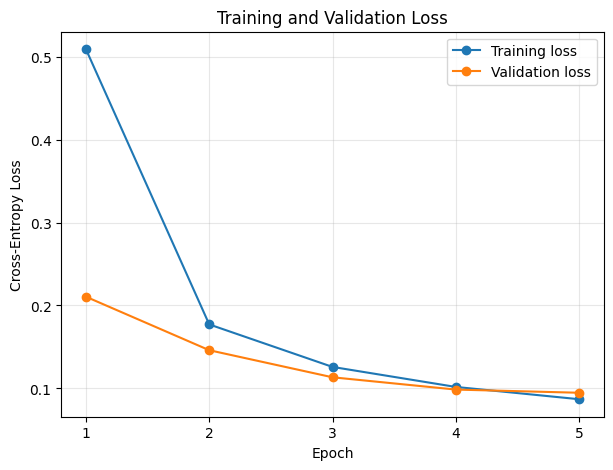
\includegraphics[width=0.58\linewidth]{fig_loss.png}
\caption{Training and validation cross-entropy loss per epoch.}
\end{figure}
\begin{figure}[H]
\centering
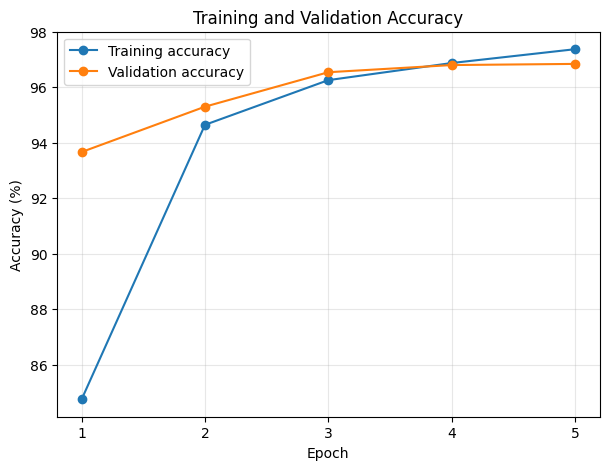
\includegraphics[width=0.58\linewidth]{fig_accuracy.png}
\caption{Training and validation accuracy per epoch.}
\end{figure}

Loss falls steadily and accuracy rises every epoch with no sign of divergence. The validation loss is lower than the training loss in the first epochs because the training loss is averaged over the whole epoch while the weights are still changing quickly, whereas validation is measured with the weights at the end of the epoch. By epoch 5 the training loss (0.0870) is slightly below the validation loss (0.0948), and the validation accuracy gain has slowed to $+0.04$ points, which suggests the model is approaching, but is not yet far into, overfitting.

% =====================================================
\section{Result Analysis, Insights, and Observations}
The selected model was evaluated once on the 10{,}000 held-out test images: \textbf{test loss 0.0856 and test accuracy 97.44\%} (256 errors). This exceeds the 94--96\% target and is close to the validation accuracy of 96.84\%, so the model generalises to unseen data.

\begin{figure}[H]
\centering
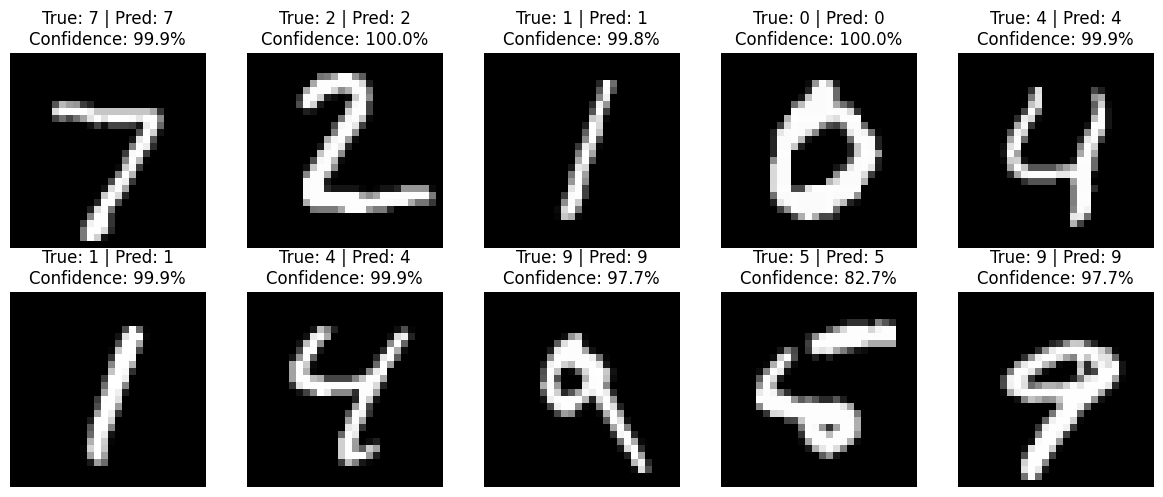
\includegraphics[width=0.85\linewidth]{fig_predictions.png}
\caption{Predictions and confidence on the first ten test images (all correct; the ``5'' is the least confident at 82.7\%).}
\end{figure}

\begin{table}[H]
\centering
\small
\begin{tabular}{@{}lcccccccccc@{}}
\toprule
\textbf{Digit} & 0 & 1 & 2 & 3 & 4 & 5 & 6 & 7 & 8 & 9 \\
\midrule
\textbf{Accuracy (\%)} & 98.9 & 98.9 & 97.8 & 98.0 & 98.6 & 98.5 & 98.3 & 96.2 & 95.0 & 94.2 \\
\bottomrule
\end{tabular}
\end{table}

\begin{figure}[H]
\centering
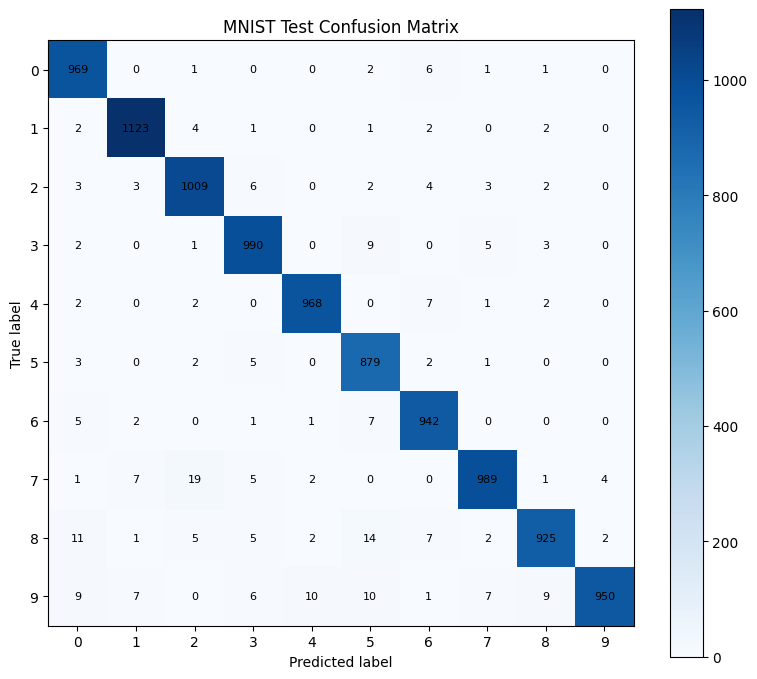
\includegraphics[width=0.6\linewidth]{fig_confusion.png}
\caption{Confusion matrix on the test set.}
\end{figure}

Digits 0 and 1 are the easiest; 9 (94.2\%), 8 (95.0\%) and 7 (96.2\%) are the hardest. The largest confusions are 7 predicted as 2 (19 images), 8 as 5 (14), 8 as 0 (11), and 9 as 5 or 4 (10 each). These are pairs of digits that can look alike in untidy handwriting, so the remaining errors look like genuinely ambiguous inputs rather than a systematic bug.

% =====================================================
\subsection{Regularisation experiment}
To measure the effect of regularisation, the same network was retrained with the same seed, data and settings, changing only one thing: \textbf{dropout ($p=0.5$) on the 128-unit hidden layer}, or \textbf{L2 weight decay ($\lambda=10^{-3}$)} on the weights. Dropout randomly sets half of the hidden activations to zero during training (the rest are scaled by $1/(1-p)$) and is switched off at validation and test time, so its training accuracy is measured with dropout on and is naturally lower.

\begin{table}[H]
\centering
\begin{tabular}{@{}lccccc@{}}
\toprule
\textbf{Model} & \textbf{Train acc} & \textbf{Val acc} & \textbf{Gap (train$-$val)} & \textbf{Test acc} & \textbf{Test loss} \\
\midrule
Baseline             & 97.37\% & 96.84\% & $+0.53\%$ & 97.44\% & 0.0856 \\
Dropout 0.5          & 94.31\% & 96.30\% & $-1.99\%$ & 96.97\% & 0.0942 \\
L2 weight decay $10^{-3}$ & 97.32\% & 96.89\% & $+0.43\%$ & 97.47\% & 0.0850 \\
\bottomrule
\end{tabular}
\end{table}

\begin{figure}[H]
\centering
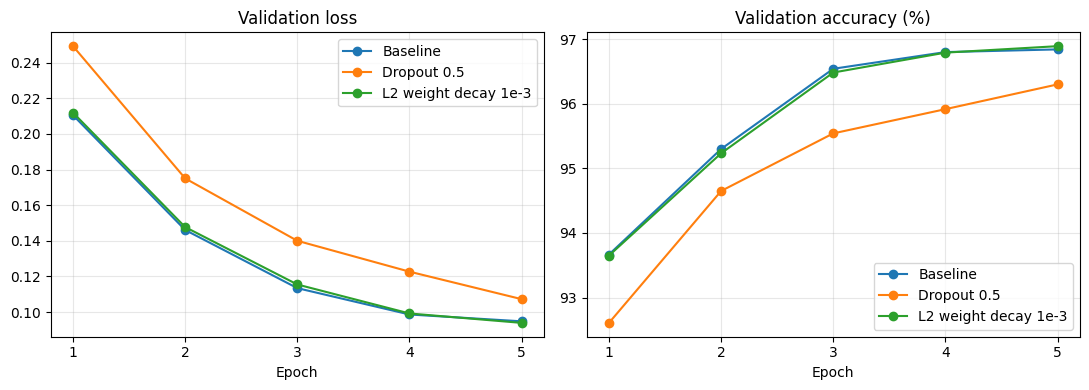
\includegraphics[width=0.95\linewidth]{fig_regularisation.png}
\caption{Validation loss and accuracy for the baseline, dropout and L2 models.}
\end{figure}

\textbf{Dropout} made training harder (training accuracy 94.31\% vs 97.37\%) and gave lower validation and test accuracy (96.97\% vs 97.44\% on the test set), with validation curves still rising at epoch 5. \textbf{L2 weight decay} gave almost identical results to the baseline: its test accuracy is 0.03 percentage points higher (3 images out of 10{,}000), which is too small to count as a real improvement. The baseline's train--validation gap is only about half a percentage point, so it is hardly overfitting after 5 epochs, and regularisation has little to correct. These are single runs with one seed, so differences of a few hundredths of a percent should not be over-interpreted; the clear effect is that dropout slows learning in this short training budget.

% =====================================================
\section{Challenges Faced and Solution Applied}
\begin{table}[H]
\centering
\small
\begin{tabularx}{\linewidth}{@{}>{\raggedright\arraybackslash}p{3.6cm} X >{\raggedright\arraybackslash}p{3.8cm}@{}}
\toprule
\textbf{Challenge} & \textbf{Solution} & \textbf{Outcome} \\
\midrule
Hand-written backprop for convolution and pooling is error-prone &
Derived each gradient ($dW$, $db$, $dx$ via col2im; pooling gradient routed to the argmax position) and verified numerically &
Gradient check: all relative errors below $2\times10^{-8}$ (Section 10b in ipynb) \\
\addlinespace
Convolution with nested Python loops is far too slow for 7{,}500 SGD steps &
Used im2col so each convolution is one matrix multiplication; col2im only loops over the 9 kernel offsets &
About 36 s per epoch on 48{,}000 images \\
\addlinespace
Overlapping patches must not lose gradient information &
col2im accumulates (\code{+=}) the gradient contributions of overlapping patches &
Gradient check passes for conv1 and conv2 \\
\addlinespace
$11{\times}11$ feature map is not divisible by 2 &
Pooling output size uses floor division ($5{\times}5$); the unused last row/column gets zero gradient &
Flatten size 400 matches the $400{\times}128$ layer; shape test passes \\

\addlinespace
Choosing which weights to report &
Saved the best-validation-accuracy weights and restored them before testing &
Selected epoch 5 (96.84\% validation); test set used only once \\
\bottomrule
\end{tabularx}
\end{table}

% =====================================================
\section{Addressing Questions}

\subsection*{Q1. Why are convolutional layers more effective than fully connected layers for image data?}
\begin{itemize}
  \item \textbf{Local connectivity:} each neuron looks at a small patch ($3{\times}3$ here), which matches how pixels relate to neighbours (strokes, edges, corners). A fully connected layer flattens the image and ignores 2-D structure.
  \item \textbf{Weight sharing:} the same kernel is applied at every position, so the layer needs very few parameters. Conv1 has only 60, whereas one fully connected layer on a $28{\times}28$ image with 128 units needs $784\cdot128+128=100{,}480$. Fewer parameters means less computation and less overfitting.
  \item \textbf{Translation invariance:} a feature such as a curve is detected wherever it appears, whereas a fully connected layer must learn each position separately.
  \item \textbf{Hierarchy of features:} stacked convolution and pooling layers build from edges to strokes to digit parts, and pooling adds tolerance to small shifts.
\end{itemize}

\subsection*{Q2. If the model achieved low accuracy, what are two possible reasons and improvements?}
\begin{itemize}
  \item \textbf{Poor optimisation settings.} A learning rate that is too small gives slow learning within 5 epochs; one that is too large makes the loss unstable; plain SGD without momentum is slow. Improve by tuning the learning rate, adding momentum or Adam, a learning-rate schedule, or more epochs. In this run the validation accuracy was still rising at epoch 5, so more epochs would probably help.
  \item \textbf{Poor initialisation or preprocessing} (un-normalised inputs, weights too small or too large causing vanishing or exploding signals or dead ReLUs). Improve by normalising the inputs and using He initialisation, both of which were used here.
  \item A further cause is \textbf{too little model capacity} (underfitting), fixed by adding filters or layers.
\end{itemize}

\subsection*{Q3. Name one regularisation technique and explain its impact.}
\textbf{Dropout} randomly zeroes a fraction of the hidden activations during training. It stops neurons from co-adapting and acts like averaging many thinned networks, which normally reduces overfitting (a smaller gap between training and validation performance). In my experiment (Section 7b) dropout 0.5 lowered training accuracy from 97.37\% to 94.31\% and test accuracy from 97.44\% to 96.97\%, and increased test loss from 0.0856 to 0.0942. So in this short 5-epoch run its impact was slightly negative: the baseline's train--validation gap was only 0.53 points, so there was little overfitting for dropout to remove, and it mainly slowed learning. Regularisation is expected to pay off with longer training or a larger model, where the gap would grow. L2 weight decay ($\lambda=10^{-3}$) had practically no effect (test accuracy 97.47\% vs 97.44\%).

% =====================================================
\section{Conclusion}
 Manually complete CNN in NumPy using im2col-based convolution, ReLU, max pooling, fully connected layers, softmax cross-entropy and mini-batch SGD with hand-derived backpropagation. The gradients were verified numerically, the best model was selected by validation accuracy, and the final model reached 97.44\% test accuracy (loss 0.0856) in five epochs. The regularisation experiment shows that dropout and L2 do not improve results in this short, barely-overfitting task.

\section*{AI use statement}
\textbf{I used Generative AI as a supporting tool during this assignment to assist with explaining neural-network concepts, reviewing the structure and readability of the code, polishing english-writing comments and documentation.}
All final content, calculations, and references are my own. AI was not used as a substitute for executing, implementing, or evaluating the model.
Examples Prompt:
    \begin{enumerate}
    \item "Explain the fundamental difference between pure SGD and mini-batch SGD. Why batch-size 32?"
    \item {"What are the good practices for storing best model weights?"}
    \item {"How to explain im2col/col2im in an academic paper?"}
    \end{enumerate}
\end{document}
